% !TeX program = xelatex
\documentclass[a4paper,10pt]{article}

% ============================================================================
% សន្លឹកកិច្ចការសិស្សបំពេញចន្លោះ ស-ខ្មៅ និងប្លង់ក្ដារខៀន/ចម្លើយគ្រូ (គ្មាន LCD / គ្មានកន្ត្រៃ)
% មេរៀនទី៦ (៥.១)៖ វិធីបូកនិងវិធីដកកន្សោមសនិទានមានភាគបែងដូចគ្នា — ត្រូវគ្នានឹង LS_Plan_RAT64.tex
% ============================================================================
\usepackage[a4paper, left=1.0cm, right=1.0cm, top=0.75cm, bottom=1.00cm, footskip=0.52cm]{geometry}
\usepackage{amsmath}
\usepackage{unicode-math}
\usepackage{fontspec}
\usepackage{array, colortbl}
\usepackage[table]{xcolor}
\usepackage{enumitem}
\usepackage{pifont}
\usepackage{fancyhdr}
\usepackage{lastpage}
\usepackage{tikz}
\usepackage[most]{tcolorbox}
\usetikzlibrary{calc, arrows.meta, decorations.pathreplacing, positioning, babel}

\makeatletter
\let\@expl@@@mark@update@singlecol@structures@@\relax
\makeatother

\providecommand{\NGSFindFonts}{%
  \IfFileExists{C:/Windows/Fonts/cambria.ttc}{%
    \def\NGSSysPath{C:/Windows/Fonts/}%
    \def\NGSUserPath{C:/Users/KIT/AppData/Local/Microsoft/Windows/Fonts/}%
  }{%
    \IfFileExists{./fonts/KhmerOSsiemreap.ttf}{\def\NGSSysPath{./fonts/}\def\NGSUserPath{./fonts/}}{%
    \IfFileExists{../fonts/KhmerOSsiemreap.ttf}{\def\NGSSysPath{../fonts/}\def\NGSUserPath{../fonts/}}{%
    \IfFileExists{../../fonts/KhmerOSsiemreap.ttf}{\def\NGSSysPath{../../fonts/}\def\NGSUserPath{../../fonts/}}{%
    \IfFileExists{../../../fonts/KhmerOSsiemreap.ttf}{\def\NGSSysPath{../../../fonts/}\def\NGSUserPath{../../../fonts/}}{%
    \IfFileExists{../../../../fonts/KhmerOSsiemreap.ttf}{\def\NGSSysPath{../../../../fonts/}\def\NGSUserPath{../../../../fonts/}}{%
    \IfFileExists{../../../../../fonts/KhmerOSsiemreap.ttf}{\def\NGSSysPath{../../../../../fonts/}\def\NGSUserPath{../../../../../fonts/}}{%
    \IfFileExists{../../../../../../fonts/KhmerOSsiemreap.ttf}{\def\NGSSysPath{../../../../../../fonts/}\def\NGSUserPath{../../../../../../fonts/}}{%
      \def\NGSSysPath{../../../../../../../fonts/}\def\NGSUserPath{../../../../../../../fonts/}%
    }}}}}}}%
  }%
}
\NGSFindFonts

\setmathfont[Path={\NGSSysPath}, FontIndex=1, Scale=1.02]{cambria.ttc}
\defaultfontfeatures{Ligatures=TeX}

\setmainfont[
  Path={\NGSUserPath}, Extension=.ttf, Script=Khmer,
  BoldFont={KhmerOSsiemreap}, BoldFeatures={FakeBold=1.8},
  ItalicFont={KhmerOSsiemreap}, ItalicFeatures={FakeSlant=0.25},
  BoldItalicFont={KhmerOSsiemreap}, BoldItalicFeatures={FakeBold=1.8, FakeSlant=0.25}
]{KhmerOSsiemreap}

\newfontfamily\muol[Path={\NGSUserPath}, Extension=.ttf, Script=Khmer]{KhmerOSmuollight}
\newfontfamily\TimesEn[Path={\NGSSysPath}, Extension=.ttf, BoldFont={timesbd}, ItalicFont={timesi}, BoldItalicFont={timesbi}]{times}
\newfontfamily\CalibriFont[Path={\NGSSysPath}, Extension=.ttf]{calibri}

\XeTeXlinebreaklocale "km"
\XeTeXlinebreakskip = 0pt plus 1pt minus 0.1pt

\definecolor{panelgray}{gray}{0.94}
\definecolor{headgray}{gray}{0.85}

\pagestyle{fancy}
\fancyhf{}
\renewcommand{\headrulewidth}{0pt}
\fancyfoot[L]{\fontsize{7.4pt}{9.5pt}\selectfont អនុវិទ្យាល័យព្រះក្រសាំង \en{|} គ្រូ៖ ហុក ប៊ុនថែន \en{|} មេរៀនទី៦ (៥.១) បូក-ដកភាគបែងដូចគ្នា \en{|} ថ្ងៃព្រហស្បតិ៍ ទី១៧ ខែធ្នូ ឆ្នាំ២០២៦}
\fancyfoot[R]{\fontsize{7.8pt}{10pt}\selectfont ទំព័រ \en{\thepage\ / \pageref{LastPage}}}

\setlength{\parindent}{0pt}
\setlength{\parskip}{0pt}
\setlength{\tabcolsep}{4pt}

\newcommand{\en}[1]{{\TimesEn #1}}
\newcommand{\enbf}[1]{{\TimesEn\bfseries #1}}
\newcommand{\unit}[1]{\,\text{\en{#1}}}
\newcommand{\riel}{\,\text{៛}}
\newcommand{\cnum}[1]{\mbox{\fontsize{10pt}{12pt}\selectfont\ding{\numexpr181+#1\relax}}}
\newcommand{\chkbox}{\tikz[baseline=-0.15ex]\draw[black, line width=0.85pt, fill=white] (0,0) rectangle (0.24cm,0.24cm);}
\newcommand{\ansbox}[1][2.0cm]{\,\tikz[baseline=-0.65ex]\draw[black, line width=0.65pt, fill=white] (0,0) rectangle (#1, 0.42cm);\,}
\newcommand{\dotline}[1][2.2cm]{\makebox[#1]{\dotfill}}

\newcommand{\pagebanner}[2]{%
  \begin{tcolorbox}[
    enhanced, sharp corners, colback=headgray, colframe=black,
    boxrule=1.05pt, boxsep=1pt, top=2.5pt, bottom=2.5pt, left=6pt, right=6pt,
    after skip=3.5pt
  ]
    {\muol\fontsize{9.0pt}{13.2pt}\selectfont #1}\hfill{\fontsize{8.0pt}{11.2pt}\selectfont\textbf{#2}}
  \end{tcolorbox}%
}

\newcommand{\secstrip}[2]{%
  \vspace{3pt}%
  \begin{tcolorbox}[
    enhanced, sharp corners, colback=panelgray, colframe=black,
    boxrule=0.8pt, boxsep=0.8pt, top=2pt, bottom=2pt, left=5pt, right=5pt,
    after skip=3pt
  ]
    {\muol\fontsize{8.5pt}{12.2pt}\selectfont #1}\hfill{\fontsize{7.8pt}{10.8pt}\selectfont\textit{#2}}
  \end{tcolorbox}%
}

\newcolumntype{L}[1]{>{\raggedright\arraybackslash}p{#1}}
\newcolumntype{C}[1]{>{\centering\arraybackslash}p{#1}}

\begin{document}
\fontsize{9.5pt}{14.5pt}\selectfont

% ============================================================================
% ទំព័រទី ១៖ សន្លឹកកិច្ចការសិស្ស (ផ្នែកមុខ៖ E1 -> E2 -> E3)
% ============================================================================
\pagebanner{សន្លឹកកិច្ចការសិស្ស \enbf{(}៦\enbf{.}៥\enbf{.}១ បូក-ដកមានភាគបែងដូចគ្នា\enbf{)} \enbf{--} ផ្នែកមុខ}{ថ្នាក់ទី៨ \en{|} ទំ.៨១}

\begin{tcolorbox}[
  enhanced, sharp corners, colback=white, colframe=black,
  boxrule=0.8pt, boxsep=1.5pt, top=3.5pt, bottom=3.5pt, left=5pt, right=5pt,
  after skip=4pt
]
  \fontsize{9.0pt}{13.0pt}\selectfont
  \textbf{ឈ្មោះសិស្ស៖} \dotline[4.3cm] \quad
  \textbf{សមាជិកក្រុម៖} \dotline[4.3cm] \quad
  \textbf{ថ្នាក់ទី៖} ៨\dotline[0.9cm] \quad
  \textbf{ក្រុមទី៖} \dotline[1.0cm]
\end{tcolorbox}

% --- E1 Engage ---
\secstrip{ផ្នែកទី ១ \enbf{(E1 - Engage)} ៖ បេសកកម្មចាប់កំហុសវង់ក្រចកពេលដកភាគយក}{រយៈពេល ៣ នាទី (គូស \ding{51} ក្នុង \chkbox)}

\begin{tcolorbox}[
  enhanced, sharp corners, colback=white, colframe=black,
  boxrule=0.8pt, boxsep=2.5pt, top=4pt, bottom=4pt, left=6pt, right=6pt
]
  គេចង់គណនាផលដក $\dfrac{a}{2a + 3} - \dfrac{a - 3}{2a + 3}$ (ទំ.៨១) ។ តើសិស្សរូបណាគណនាបានត្រឹមត្រូវ?\\[3pt]
  \chkbox\ \textbf{សិស្ស ក៖} $\dfrac{a - a - 3}{2a + 3} = -\dfrac{3}{2a + 3}$ \qquad
  \chkbox\ \textbf{សិស្ស ខ៖} $\dfrac{a - (a - 3)}{2a + 3} = \dfrac{a - a + 3}{2a + 3} = \dfrac{3}{2a + 3}$\\[3pt]
  $\bullet$ \textbf{តេស្តដោយជំនួស $a = 1$៖} កន្សោមដើមស្មើ $\dfrac{1}{5} - \dfrac{-2}{5} = \dfrac{3}{5}$; \ ចម្លើយសិស្ស ក ស្មើ \ansbox[1.7cm]; \ សិស្ស ខ ស្មើ \ansbox[1.7cm] ។
\end{tcolorbox}

\vspace{3pt}

% --- E2 Explore ---
\secstrip{ផ្នែកទី ២ \enbf{(E2 - Explore)} ៖ ភាគបែងដូចគ្នា និងការប្ដូរភាគបែងផ្ទុយ (ទំ.៨១)}{រយៈពេល ១១ នាទី}

\textbf{សកម្មភាព ១ (\en{E2-A} — ៥ នាទី)៖ ភាគបែងដូចគ្នា និងការសម្រួលចម្លើយ (ទំ.៨១ ឧទាហរណ៍ ក, ខ, គ)}

\begin{tcolorbox}[
  enhanced, sharp corners, colback=white, colframe=black,
  boxrule=0.8pt, boxsep=2.5pt, top=4pt, bottom=4pt, left=6pt, right=6pt
]
  $\bullet$ \textbf{១) ឧទាហរណ៍ ក, ខ៖} ក) $\dfrac{5}{a} + \dfrac{7}{a} =$ \ansbox[2.2cm] \qquad
  ខ) $\dfrac{3y - 2}{y - 5} + \dfrac{8y + 7}{y - 5} =$ \ansbox[3.0cm]\\[4pt]
  $\bullet$ \textbf{២) ឧទាហរណ៍ គ៖} $\dfrac{3x}{(x-1)(x-2)} - \dfrac{6}{(x-1)(x-2)} = \dfrac{3(x - 2)}{(x-1)(x-2)} =$ \ansbox[2.8cm]
\end{tcolorbox}

\vspace{4pt}
\textbf{សកម្មភាព ២ (\en{E2-B} — ៦ នាទី)៖ ភាគបែងផ្ទុយ $3 - x = -(x - 3)$ និងដកពហុធា (ទំ.៨១ លំហាត់គំរូ ក, ខ)}

\begin{tcolorbox}[
  enhanced, sharp corners, colback=white, colframe=black,
  boxrule=0.8pt, boxsep=2.5pt, top=4pt, bottom=4pt, left=6pt, right=6pt
]
  $\bullet$ \textbf{១) គំរូ ក៖} $\dfrac{2}{x - 3} + \dfrac{7}{3 - x} = \dfrac{2}{x - 3} - \dfrac{7}{x - 3} = \dfrac{2 - 7}{x - 3} =$ \ansbox[2.8cm]\\[4pt]
  $\bullet$ \textbf{២) គំរូ ខ៖} $\dfrac{a}{2a + 3} - \dfrac{a - 3}{2a + 3} = \dfrac{a - (a - 3)}{2a + 3} =$ \ansbox[2.8cm]
\end{tcolorbox}

\vfill

% --- E3 Explain ---
\secstrip{ផ្នែកទី ៣ \enbf{(E3 - Explain)} ៖ សង្ខេបវិធានបូក-ដក និងធនាគារហេតុផល \enbf{B\&W}}{រយៈពេល ៦ នាទី}

\begin{tcolorbox}[
  enhanced, sharp corners, colback=white, colframe=black,
  boxrule=0.85pt, boxsep=2.5pt, top=4pt, bottom=4pt, left=6pt, right=6pt
]
  $\bullet$ \textbf{១) វិធានជាទូទៅ ($B \neq 0$)៖} $\dfrac{A}{B} + \dfrac{C}{B} =$ \ansbox[2.2cm] \quad និង \quad $\dfrac{A}{B} - \dfrac{C}{B} =$ \ansbox[2.4cm]\\[4pt]
  $\bullet$ \textbf{២) ភាគបែងផ្ទុយ៖} ដោយ $b - a = -(a - b)$ គេបាន $+\dfrac{C}{b - a} =$ \ansbox[2.0cm] និង $-\dfrac{C}{b - a} =$ \ansbox[2.0cm]\\[4pt]
  \tikz\draw[black, dashed, line width=0.6pt] (0,0) -- (\linewidth,0);\\[3pt]
  \fontsize{8.8pt}{13.0pt}\selectfont
  \textbf{ធនាគារហេតុផល (\en{Warrant Bank})៖} \quad
  \cnum{1} រក្សាភាគបែងរួមដដែល (ហាមបូក-ដកភាគបែង)\\
  \cnum{2} ដាក់វង់ក្រចកការពារផលដក $A - (C)$ \quad
  \cnum{3} ប្ដូរភាគបែងផ្ទុយ $b-a = -(a-b)$ \quad
  \cnum{4} សម្រួលលទ្ធផលចុងក្រោយបើអាច
\end{tcolorbox}

% ============================================================================
% ទំព័រទី ២៖ សន្លឹកកិច្ចការសិស្ស (ផ្នែកខាងខ្នង៖ E4 -> E5 -> កិច្ចការផ្ទះ)
% ============================================================================
\clearpage
\pagebanner{សន្លឹកកិច្ចការសិស្ស \enbf{(}៦\enbf{.}៥\enbf{.}១ បូក-ដកមានភាគបែងដូចគ្នា\enbf{)} \enbf{--} ផ្នែកខ្នង}{ថ្នាក់ទី៨ \en{|} ទំ.៨១, ៨៦}

% --- E4 Elaborate ---
\secstrip{ផ្នែកទី ៤ \enbf{(E4 - Elaborate)} ៖ ប្រតិបត្តិ ក, ខ (ទំ.៨១) និងលំហាត់ ទំ.៨៦ \enbf{\#7} ឆ}{រយៈពេល ១០ នាទី}

\begin{tcolorbox}[
  enhanced, sharp corners, colback=white, colframe=black,
  boxrule=0.8pt, boxsep=2.5pt, top=4pt, bottom=4pt, left=6pt, right=6pt
]
  \textbf{១) ប្រតិបត្តិ ក (ទំ.៨១) និង \en{\#7} ឆ (ទំ.៨៦)៖}\\[3pt]
  \hspace*{0.3cm}$\bullet$ ប្រតិបត្តិ ក៖ $\dfrac{t^2}{t + 4} + \dfrac{4t}{t + 4} =$ \ansbox[2.4cm] \qquad
  \en{\#7} ឆ៖ $\dfrac{a^2}{a - b} + \dfrac{-b^2}{a - b} =$ \ansbox[2.8cm]\\[4pt]
  \textbf{២) ប្រតិបត្តិ ខ (ទំ.៨១ — ភាគបែងផ្ទុយ)៖} $\dfrac{5x}{x - y} - \dfrac{5y}{y - x} = \dfrac{5x}{x - y} + \dfrac{5y}{x - y} =$ \ansbox[3.2cm]\\[4pt]
  \textbf{ឆ្លុះបញ្ចាំង (\en{EIA Looking-Back})៖} ហេតុអ្វី $-\dfrac{5y}{y - x}$ ក្លាយជា $+\dfrac{5y}{x - y}$? \dotline[4.2cm] ។
\end{tcolorbox}

\vspace{4pt}

% --- E5 Evaluate ---
\secstrip{ផ្នែកទី ៥ \enbf{(E5 - Evaluate)} ៖ ប្រតិបត្តិ (ទំ.៨៦ \enbf{\#7}) សំណួរវិនិច្ឆ័យ \enbf{A--D} និងសំបុត្រចេញ}{រយៈពេល ១០ នាទី}

\begin{tcolorbox}[
  enhanced, sharp corners, colback=white, colframe=black,
  boxrule=0.8pt, boxsep=2.5pt, top=4pt, bottom=4pt, left=6pt, right=6pt
]
  \textbf{១) ប្រតិបត្តិជាក្រុម (ទំ.៨៦ លេខ ៧ ក, គ, ង)៖}\\[3pt]
  \hspace*{0.3cm}$\bullet$ \en{\#7} ក៖ $\dfrac{12a}{7} + \dfrac{2a}{7} =$ \ansbox[2.2cm] \quad
  \en{\#7} គ៖ $\dfrac{x}{x - 1} + \dfrac{1}{x - 1} =$ \ansbox[2.6cm] \quad
  \en{\#7} ង៖ $\dfrac{6x}{x + y} + \dfrac{6y}{x + y} =$ \ansbox[2.0cm]\\[4pt]
  \textbf{២) បិទបេសកកម្ម \en{E1}៖} សិស្ស \dotline[1.1cm] ត្រឹមត្រូវ ព្រោះចំពោះ $a = 1$ បាន $\dfrac{3}{2(1)+3} =$ \ansbox[1.8cm] ត្រូវនឹងកន្សោមដើម ។
\end{tcolorbox}

\vspace{4pt}

\begin{tcolorbox}[
  enhanced, sharp corners, colback=white, colframe=black,
  boxrule=0.85pt, boxsep=2.5pt, top=4pt, bottom=4pt, left=6pt, right=6pt
]
  \textbf{៣) សំណួរវិនិច្ឆ័យ \en{A--D} (គណនាផលដក $\dfrac{2x}{x - 4} - \dfrac{x + 4}{x - 4}$ — គូសរង្វង់ រួចលើកម្រាមដៃ ១--៤)៖}\\[3pt]
  \textbf{\en{A.}} $\dfrac{x + 4}{x - 4}$ \qquad\qquad\quad
  \textbf{\en{B.}} $1$ \qquad\qquad\quad
  \textbf{\en{C.}} $0$ \qquad\qquad\quad
  \textbf{\en{D.}} $\dfrac{3x + 4}{x - 4}$\\[4pt]
  \tikz\draw[black, dashed, line width=0.6pt] (0,0) -- (\linewidth,0);\\[3pt]
  \textbf{៤) សំបុត្រចេញ ៦០ វិនាទី (ទំ.៨៦ \en{\#7} ជ)៖} គណនា $\dfrac{a}{2a - 2b} - \dfrac{b}{2a - 2b} =$ \ansbox[3.0cm] ។
\end{tcolorbox}

\vfill

% --- Homework Box ---
\begin{tcolorbox}[
  enhanced, sharp corners, colback=panelgray, colframe=black,
  boxrule=0.9pt, boxsep=2.5pt, top=4pt, bottom=4pt, left=6pt, right=6pt
]
  {\muol\fontsize{8.8pt}{13pt}\selectfont កិច្ចការផ្ទះ \enbf{(}សៀវភៅគោល ទំ\enbf{.}៨៦ លេខ ៧ ខ\enbf{,} ឃ\enbf{,} ច\enbf{,} ឈ\enbf{)}}\\[3pt]
  $\bullet$ \textbf{១) ទំ.៨៦ \en{\#7} ខ, ឃ៖} គណនា $\dfrac{y}{14} - \dfrac{3y}{14}$ និង $\dfrac{y}{b + 6} + \dfrac{2y}{b + 6}$ ។\\[2pt]
  $\bullet$ \textbf{២) ទំ.៨៦ \en{\#7} ច, ឈ៖} គណនា $\dfrac{a + b}{x - 3} - \dfrac{a + b}{3 - x}$ និង $\dfrac{x^2}{x^2 - 1} + \dfrac{2x + 1}{x^2 - 1}$ ។
\end{tcolorbox}

% ============================================================================
% ទំព័រទី ៣៖ ទំព័រគ្រូបង្រៀន — ប្លង់ក្ដារខៀន ៣ ផ្នែក (គ្មាន LCD) និងចម្លើយផ្ទៀងផ្ទាត់រហ័ស
% ============================================================================
\clearpage
\pagebanner{ទំព័រគ្រូបង្រៀន ៖ ប្លង់ក្ដារខៀន \enbf{(}គ្មាន \enbf{LCD)} និងចម្លើយផ្ទៀងផ្ទាត់រហ័ស}{៦.៥.១ បូក-ដកមានភាគបែងដូចគ្នា (\en{RAT64})}

\secstrip{១. គំរូប្លង់បែងចែកក្ដារខៀន ៣ ផ្នែក សម្រាប់ថ្នាក់រៀនគ្មាន \enbf{LCD}}{សម្រាប់គ្រូប្រើដីស/ហ្វឺត}

\begin{center}
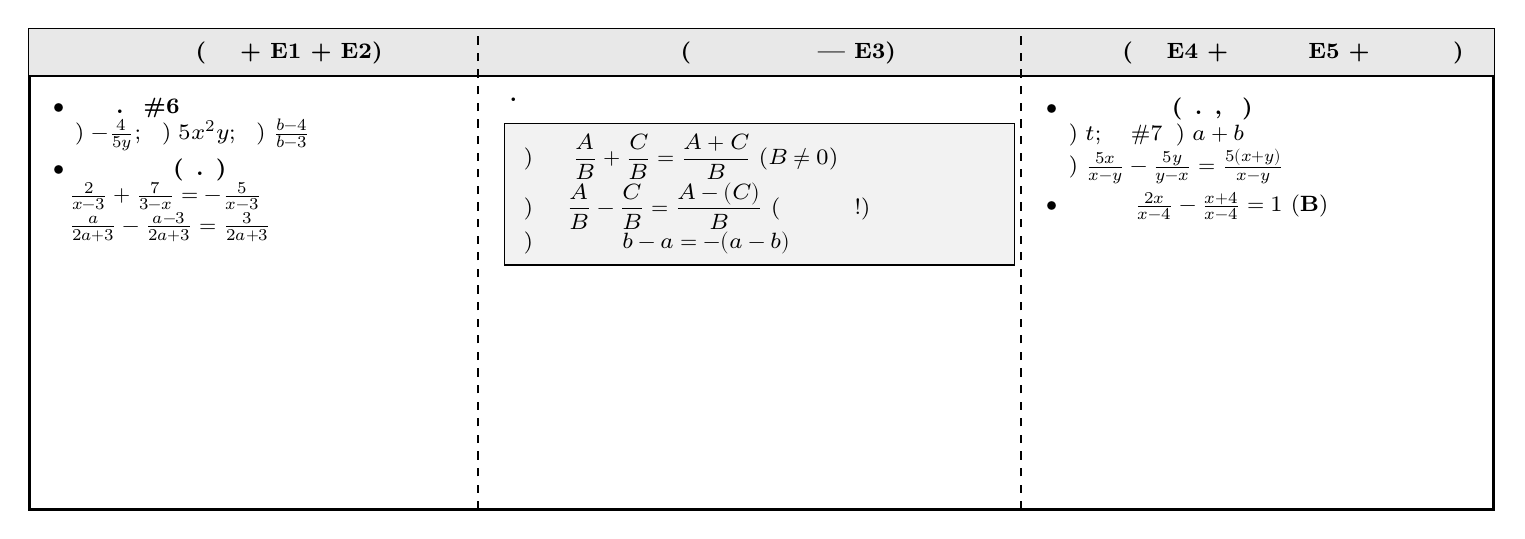
\begin{tikzpicture}[x=1cm, y=1cm, every node/.style={font=\footnotesize, text=black}]
  \draw[black, line width=1.1pt] (0,0) rectangle (18.6,6.1);
  \fill[gray!18] (0,5.50) rectangle (18.6,6.1);
  \draw[black, line width=0.7pt] (0,5.50) -- (18.6,5.50);
  \draw[black, dashed, line width=0.75pt] (5.7,0) -- (5.7,6.1);
  \draw[black, dashed, line width=0.75pt] (12.6,0) -- (12.6,6.1);

  \node at (2.85,5.80) {\textbf{ផ្នែកឆ្វេង (កំណែ + \en{E1} + \en{E2})}};
  \node at (9.15,5.80) {\textbf{ផ្នែកកណ្ដាល (ខ្លឹមសារគោលរក្សាទុក — \en{E3})}};
  \node at (15.60,5.80) {\textbf{ផ្នែកស្ដាំ (គំរូ \en{E4} + ប្រតិបត្តិ \en{E5} + កិច្ចការផ្ទះ)}};

  % Left zone
  \node[anchor=north west, text width=5.3cm] at (0.18,5.35) {
    $\bullet$ \textbf{កំណែ ទំ.៨៦ \en{\#6}៖}\\
    \hspace*{0.2cm}ក) $-\tfrac{4}{5y}$; \ ខ) $5x^2y$; \ ដ) $\tfrac{b-4}{b-3}$\\[2pt]
    $\bullet$ \textbf{ឧទាហរណ៍ និងគំរូ (ទំ.៨១)៖}\\
    \hspace*{0.2cm}$\tfrac{2}{x-3} + \tfrac{7}{3-x} = -\tfrac{5}{x-3}$\\
    \hspace*{0.2cm}$\tfrac{a}{2a+3} - \tfrac{a-3}{2a+3} = \tfrac{3}{2a+3}$
  };

  % Center zone
  \node[anchor=north west, text width=6.5cm] at (5.90,5.35) {
    {\muol\fontsize{8.0pt}{12pt}\selectfont ៥\enbf{.}១ បូកនិងដកមានភាគបែងដូចគ្នា}\\[3pt]
    \begin{tcolorbox}[enhanced, sharp corners, colback=gray!10, colframe=black, boxrule=0.6pt, boxsep=1.5pt, left=3pt, right=3pt, top=2pt, bottom=2pt]
      ១) \textbf{បូក៖} $\dfrac{A}{B} + \dfrac{C}{B} = \dfrac{A + C}{B}$ ($B \neq 0$)\\
      ២) \textbf{ដក៖} $\dfrac{A}{B} - \dfrac{C}{B} = \dfrac{A - (C)}{B}$ (ដាក់វង់ក្រចក!)\\
      ៣) \textbf{ភាគបែងផ្ទុយ៖} $b - a = -(a - b)$
    \end{tcolorbox}
  };

  % Right zone
  \node[anchor=north west, text width=5.6cm] at (12.80,5.35) {
    $\bullet$ \textbf{ប្រតិបត្តិពង្រីក (ទំ.៨១, ៨៦)៖}\\
    \hspace*{0.2cm}ក) $t$; \quad \en{\#7} ឆ) $a + b$\\
    \hspace*{0.2cm}ខ) $\tfrac{5x}{x-y} - \tfrac{5y}{y-x} = \tfrac{5(x+y)}{x-y}$\\[2pt]
    $\bullet$ \textbf{វិនិច្ឆ័យ៖} $\tfrac{2x}{x-4} - \tfrac{x+4}{x-4} = 1$ (\textbf{\en{B}})
  };
\end{tikzpicture}
\end{center}

\secstrip{២. ចម្លើយផ្ទៀងផ្ទាត់រហ័សសម្រាប់សន្លឹកកិច្ចការសិស្ស \enbf{(}ទំព័រ ១ និង ទំព័រ ២\enbf{)}}{\en{Answer Key}}

\begin{tcolorbox}[
  enhanced, sharp corners, colback=white, colframe=black,
  boxrule=0.8pt, boxsep=2.5pt, top=4pt, bottom=4pt, left=6pt, right=6pt
]
  $\bullet$ \textbf{ផ្នែក \en{E1}៖} សិស្ស ខ ត្រឹមត្រូវ (តេស្ត $a=1$៖ សិស្ស ក បាន $-\tfrac{3}{5} \neq \tfrac{3}{5}$; សិស្ស ខ បាន $\tfrac{3}{5}$ ត្រឹមត្រូវ) ។\\[2pt]
  $\bullet$ \textbf{ផ្នែក \en{E2}៖} សកម្មភាព ១៖ $\tfrac{12}{a}$; $\tfrac{11y+5}{y-5}$; $\tfrac{3}{x-1}$ ។ សកម្មភាព ២៖ $-\tfrac{5}{x-3}$; $\tfrac{3}{2a+3}$ ។\\[2pt]
  $\bullet$ \textbf{ផ្នែក \en{E4}៖} ១) $t$; $a + b$; ២) $\tfrac{5(x+y)}{x-y}$ (ព្រោះ $y-x = -(x-y)$ ដកជួបដកបានបូក) ។\\[2pt]
  $\bullet$ \textbf{ផ្នែក \en{E5}៖} ១) $2a$; $\tfrac{x+1}{x-1}$; $6$; ២) សិស្ស ខ ($\tfrac{3}{5}$); ៣) \textbf{ជម្រើស \en{B}} ($1$); ៤) $\tfrac{1}{2}$ ។
\end{tcolorbox}

\secstrip{៣. ចម្លើយលម្អិតនៃកិច្ចការផ្ទះ \enbf{(}សម្រាប់គ្រូផ្ទៀងផ្ទាត់នៅដើមម៉ោងបន្ទាប់\enbf{)}}{សៀវភៅគោល ទំ.៨៦}

\begin{tcolorbox}[
  enhanced, sharp corners, colback=white, colframe=black,
  boxrule=0.8pt, boxsep=2.5pt, top=4pt, bottom=4pt, left=6pt, right=6pt
]
  $\bullet$ \textbf{១) ទំ.៨៦ \en{\#7} ខ, ឃ៖} ខ) $\dfrac{-2y}{14} = \mathbf{-\dfrac{y}{7}}$; \quad ឃ) $\dfrac{y + 2y}{b + 6} = \mathbf{\dfrac{3y}{b + 6}}$ ។\\[2pt]
  $\bullet$ \textbf{២) ទំ.៨៦ \en{\#7} ច, ឈ៖} ច) $\dfrac{a+b}{x-3} + \dfrac{a+b}{x-3} = \mathbf{\dfrac{2(a + b)}{x - 3}}$; \quad ឈ) $\dfrac{(x + 1)^2}{(x - 1)(x + 1)} = \mathbf{\dfrac{x + 1}{x - 1}}$ ។
\end{tcolorbox}

\end{document}
